\chapter{经济性数据库}\label{database}

尽管商用航空领域经济性研究的重要性得到广泛认可,但开展经济性分析模型和方法研究所需要的数据的获取并非易事,部分的原因在于相关利益方对经济性数据的获取、处理和公布过程存在差异,导致公开的数据之间存在较大的差异,也并非所有的研究者都可以方便的获取商业数据库的数据。因此,开展航空经济性研究需要解决的一个重要问题是数据来源,数据收集、处理和验证问题。这是建立各种经济性分析模型的基础。


民机设计除了要满足航空公司对飞机安全性及性能的要求,对乘客具有吸引力外,还必须能够为航空公司带来经济效益。通过增加飞机的销售数量,飞机制造商可以收回投入的项目开发成本,并通过进一步的利润积累为新技术的研究和下一代飞机的研发提供资金。因此成功的机型除了技术上的先进性以外,还需要具有良好的经济性,包括较低的购买成本和使用成本等。

民机的经济性分析是总体设计的重要内容,对整个项目的市场成功具有至关重要的作用。飞机项目,尤其是全新的飞机项目的研发时间往往很长,其累计现金流在设计初期直到设计定型,将产品推向市场并获得初始订单之前,一直都为负值。在销售的飞机达到一定数目时才可以收回研发及生产成本,亦即达到盈亏平衡点。由于其所需的巨额的现金投入,使飞机项目的风险巨大。在飞机设计的各个阶段,要对设计方案的经济性和市场前景进行尽可能准确的分析和预测,以增加项目成功的几率。这一任务在设计的初期尤其重要,这一阶段作出的设计决策对飞机的购买成本及使用成本的影响巨大。

\section{数据来源}

一些典型的数据来源包括IATA

\section{成本概念与评估方法}
%航空公司对飞机的经济性的评估通常会考虑下面几个方面的成本
%\begin{itemize}
%\item[-]资本成本-购买飞机的成本,亦即飞机的价格
%\item[-]直接使用成本-使用飞机进行商业运营的成本
%\item[-]间接使用成本-维持航空公司运营的成本
%\item[-]总使用成本-提供商业航空服务的所有成本
%\item[-]每座公里成本-平均到每座位公里的成本
%\end{itemize}

\subsection{全寿命使用成本}

航空公司使用一架飞机完成特定航线任务涉及三个方面的成本,飞机的购买成本、使用成本和支撑飞机使用的成本,如维修和备件成本等。而一架飞机从下线和投入航线运营,到最后退役所经历的时间长达$20\sim30$年。

全寿命周期成本应该包括与飞机直接相关的成本和支撑飞机运行的非直接成本。非直接成本的计算与航空公司的运行方式和财务计算方法有直接的关系,不同航空公司的计算方法得出的结果差异比较大。

Curren等提出了将基于一般性规则与偶然性因素(Genetic-Casual)相结合的方法用于制造成本和全寿命周期成本的估算研究中~\cite{curren05}。Scholz 提出了与常规DOC方法略有区别的DOC$_{\textrm{sys}}$方法~\cite{scholz},与传统DOC计算的主要区别是加入了针对飞机系统进行评估的有关方法,将能够区别不同飞机的成本都记入DOC$_{\textrm{sys}}$,例如在对比两人机组飞机时,可以将机组成本忽略,而将原本分类为IOC的维持备用件库存所发生的成本记入直接使用成本。

民机的总使用成本(TOC)主要由以下几个元素构成,包括与飞机有关的使用成本(Airplane Related Operating Cost AROC),或称直接使用成本(DOC);与乘客服务有关的使用成本;与货运服务有关的使用成本;与飞机地面系统有关的使用成本等,其中后面三个方面的内容也统称为间接使用成本(IOC),非直接成本在总的使用成本中大约占$15\%\sim50\%$,在缺乏可靠数据估算的情况下,可以假定IOC的数值近似等同于为DOC,而将重点放在DOC的计算上。DOC中又包括两个方面的内容:所有权成本或资本成本,和现金使用成本(CAROC)。具体的划分如图\ref{fig_toc}所示。
\begin{figure}
\begin{center}
  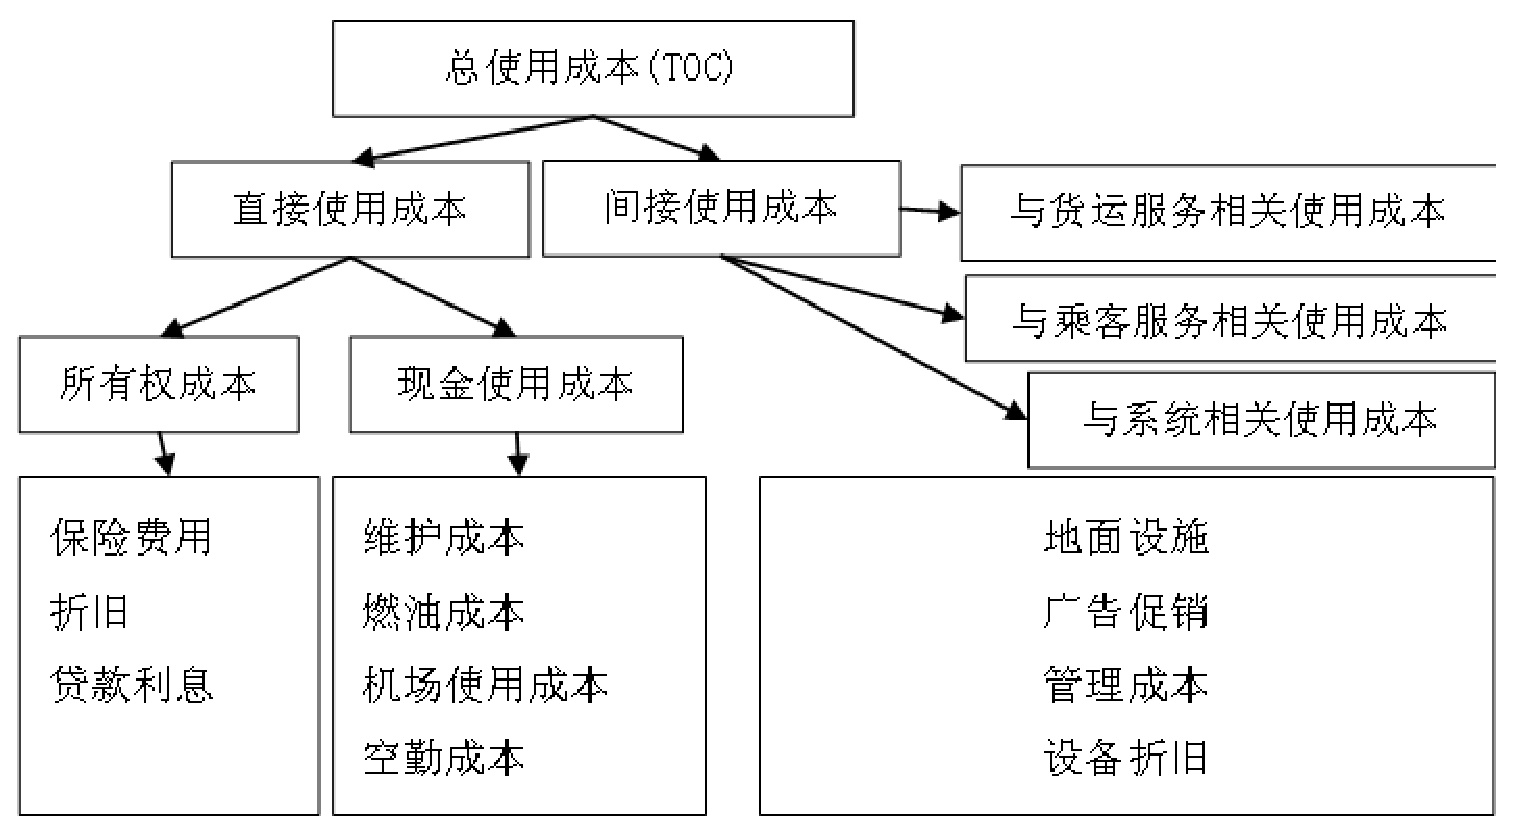
\includegraphics[width=0.8\textwidth]{doc/toc_composition.eps}
  \caption{飞机总的使用经济性(TOC)的构成}
  \label{fig_toc}
\end{center}
\end{figure}

飞机的经济性可以使用下述不同的指标进行衡量,反映飞机直接使用成本的指
标有:
\begin{itemize}
\item[(1)]飞行小时成本(DOC美元/飞行小时)
\item[(2)]航段成本(DOC美元/航段)
\item[(3)]座海里成本(DOC美元/座海里)
\item[(4)]吨海里成本(DOC美元/吨海里)
\end{itemize}
反映飞机制造成本的指标包括:
\begin{itemize}
\item[(1)]单位空机成本(美元/$W_{oe}$)
\item[(2)]单位商载成本(美元/$W_{pl}$)
\end{itemize}

式中,$W_{oe}$和$W_{pl}$分别为使用空机重量(吨)和最大使用商载重量(吨)。其中,最常用的是民机经济性评价指标是座海里成本。

\subsection{经济性评估方法}
经济性评估可以使用不同的经济性指标进行。准确估算飞机的经济性是一项非常困难的工作,却又是概念设计和初步设计阶段一项非常重要的工作。在这一阶段有关设计方案的数据非常缺乏,众多参数都有待确定。这又为准确估算飞机成本带来了很大的困难。

飞机成本估算的常用方法包括自下而上的方法,从估算零件的成本到整个产品的成本,其中涉及对大量数据的处理,而估算的结果受到多种因素的影响,在概念设计阶段,当许多细节尚未确定时,很难采用这种方法。

第二种方法是基于历史数据进行类比分析来进行估算,这种方法对新飞机研发成本的估算存在很大困难,尤其是当飞机间的技术水平差距较大时,需要采用合适的修正因子。可以利用的方法包括案例推理(Case-Based Reasoning, CBR)以及使用神经网络和模糊逻辑的工具等。

第三种方法通过建立成本与关键设计参数间的关联关系来进行,因而称为“参数法”(Parametric Costing)。将DOC和设计参数进行关联得到的成本模型与重量、性能、几何等模块相集成,进行各种设计参数对经济性影响的灵敏度研究,是目前越来越多采用的方法。

其他在财务分析领域使用的方法包括作业成本法(Activity-Based Costing,ABC)和薄利成本法(Lean Costing),这些方法代表了另一类将成本与资源使用和工程活动进行映射的方法。随着计算建模技术,特别是CAD技术的发展,初步设计阶段可以使用越来越多的详细数据,这一发展趋势使得对部件的制造成本信息的把握越来越准确,尤其是对传统金属类结构形式。多种成本估算方法相结合,能够为初始设计阶段的有效决策提供更多的依据。

